\documentclass[12pt]{article}

% This first part of the file is called the PREAMBLE. It includes
% customizations and command definitions. The preamble is everything
% between \documentclass and \begin{document}.

\usepackage[margin=1in]{geometry}  % set the margins to 1in on all sides
\usepackage{graphicx}              % to include figures
\usepackage{amsmath}               % great math stuff
\usepackage{amsfonts}              % for blackboard bold, etc
\usepackage{amsthm}                % better theorem environments
\usepackage{amssymb} 
\usepackage{mathptmx}
\usepackage{enumerate}
\usepackage{graphicx}
\usepackage{listings}
\usepackage{xcolor}

% various theorems, numbered by section

\newtheorem{thm}{Theorem}[section]
\newtheorem{lem}[thm]{Lemma}
\newtheorem{prop}[thm]{Proposition}
\newtheorem{cor}[thm]{Corollary}
\newtheorem{conj}[thm]{Conjecture}
\newtheorem{mydef}[thm]{Definition}
\lstset{
	basicstyle          =   \sffamily,          
	keywordstyle        =   \bfseries,          
	commentstyle        =   \rmfamily\itshape,  
	stringstyle         =   \ttfamily,  
	flexiblecolumns,                
	numbers             =   left,   
	showspaces          =   false,  
	numberstyle         =   \fontsize{5}{skip},    
	showstringspaces    =   false,
	captionpos          =   t,      
	frame               =   lrtb,   
}

\lstdefinestyle{cpp}{
	language        =   cpp, 
	basicstyle      =   \fontsize{5}{skip},
	numberstyle     =   \fontsize{5}{skip},
	keywordstyle    =   \color{blue},
	keywordstyle    =   [2] \color{teal},
	stringstyle     =   \color{magenta},
	commentstyle    =   \color{red}\ttfamily,
	breaklines      =   true,   
	columns         =   fixed,  
	basewidth       =   0.5em,
}
\begin{document}


\title{ CSE 120 Spring 2021\\
	Homework Assignment 1}

\author{Jaden Liu \\
	zliu259@ucsc.edu\\ 
University of California at Santa Cruz\\
Santa Cruz, CA 95064 USA }

\maketitle


\section{HW1} 
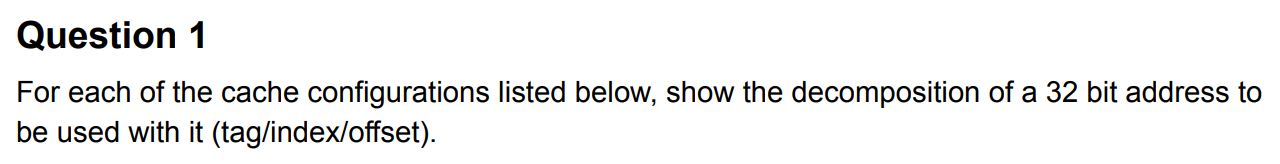
\includegraphics[scale=0.37]{q1_q.png}\\
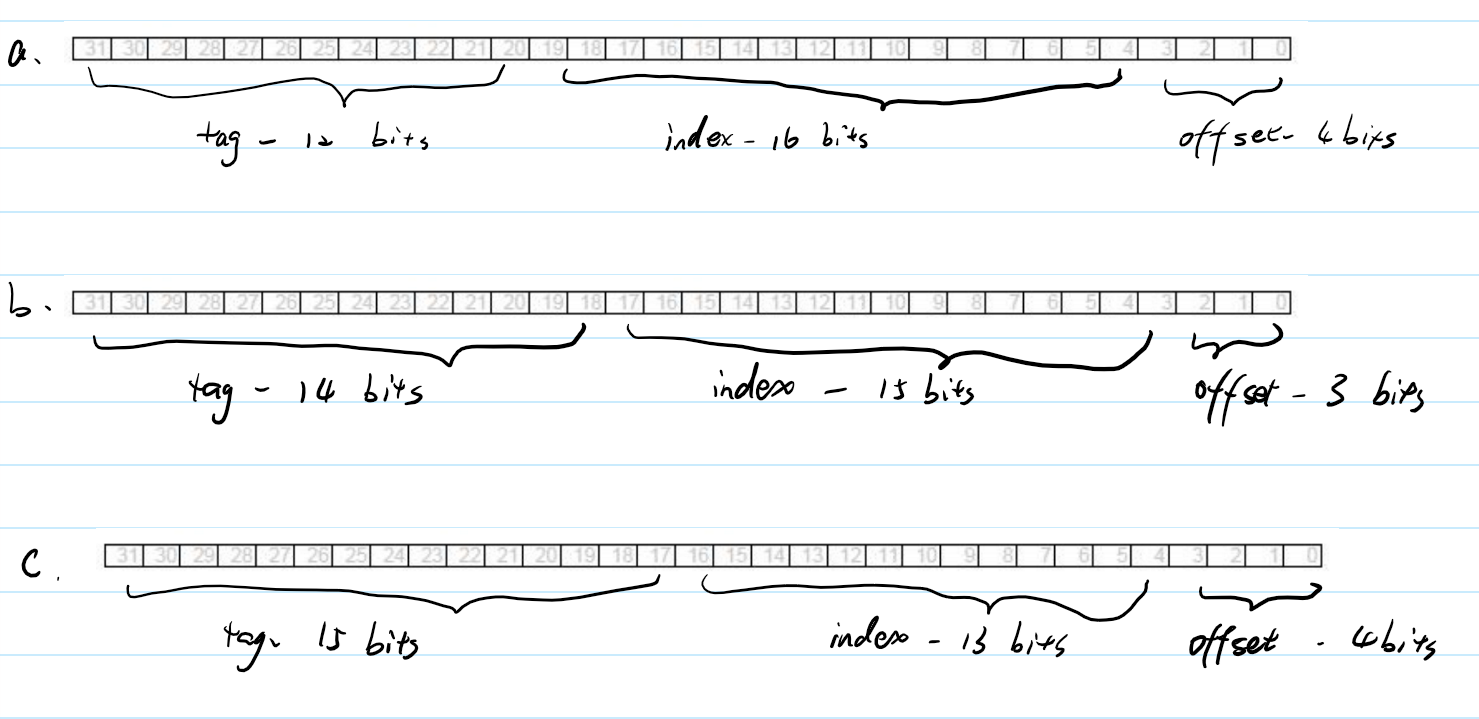
\includegraphics[scale=0.3]{q1.png}\\
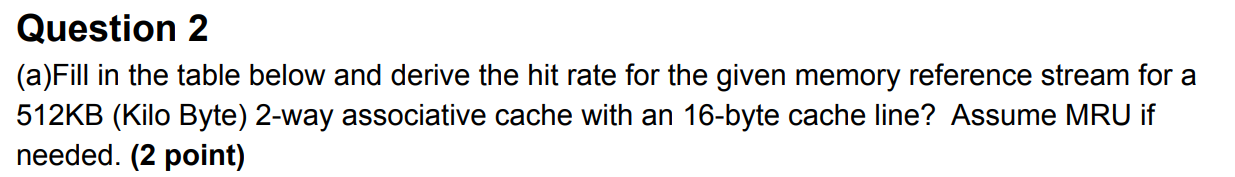
\includegraphics[scale=0.37]{q2_q1.png}\\
\begin{proof}[Solution for a]
	\ \\
	\begin{tabular}{lllll}
		Memory Address & Tag   & Index & Byte  & Hit/Miss \\
		0x1234AB22 & 0x48D & 0xAB2 & 0x2   & Miss \\
		0x1234AB20 & 0x48D & 0xAB2 & 0x0   & Hit \\
		0x1234D020 & 0x48D & 0xD02 & 0x0   & Miss \\
		0x1234D02F & 0x48D & 0xD02 & 0xF   & Hit \\
		0x1234AB26 & 0x48D & 0xAB2 & 0x6   & Hit \\
		0x1234AB33 & 0x48D & 0xAB3 & 0x3   & Miss \\
		0x1234D023 & 0x48D & 0xD02 & 0x3   & Hit \\
		0x1234D02B & 0x48D & 0xD02 & 0xB   & Hit \\
		0x1234AB22 & 0x48D & 0xAB2 & 0x2   & Hit \\
		0x1234AB28 & 0x48D & 0xAB2 & 0x8   & Hit \\
	\end{tabular}\\
Hit rate = 7/10
\end{proof}
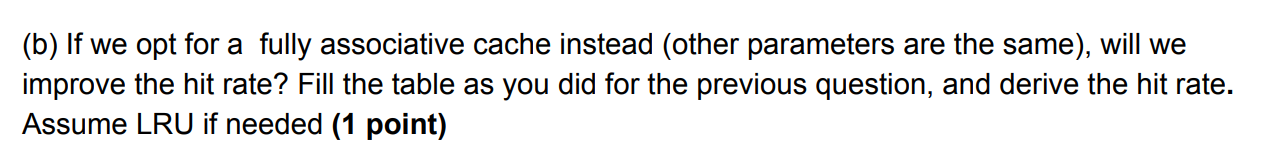
\includegraphics[scale=0.37]{q2_q2.png}\\
\begin{proof}[Solution for b]
	\ \\
	 \begin{tabular}{lllll}
		Memory Address & Tag   & Index & Byte  & Hit/Miss \\
		0x1234AB22 & 0x1234AB2 & -     & 0x2   & Miss \\
		0x1234AB20 & 0x1234AB2 & -     & 0x0   & Hit \\
		0x1234D020 & 0x1234D02 & -     & 0x0   & Miss \\
		0x1234D02F & 0x1234D02 & -     & 0xF   & Hit \\
		0x1234AB26 & 0x1234AB2 & -     & 0x6   & Hit \\
		0x1234AB33 & 0x1234AB3 & -     & 0x3   & Miss \\
		0x1234D023 & 0x1234D02 & -     & 0x3   & Hit \\
		0x1234D02B & 0x1234D02 & -     & 0xB   & Hit \\
		0x1234AB22 & 0x1234AB2 & -     & 0x2   & Hit \\
		0x1234AB28 & 0x1234AB2 & -     & 0x8   & Hit \\
	\end{tabular}\\
	Hit rate = 7/10
\end{proof}
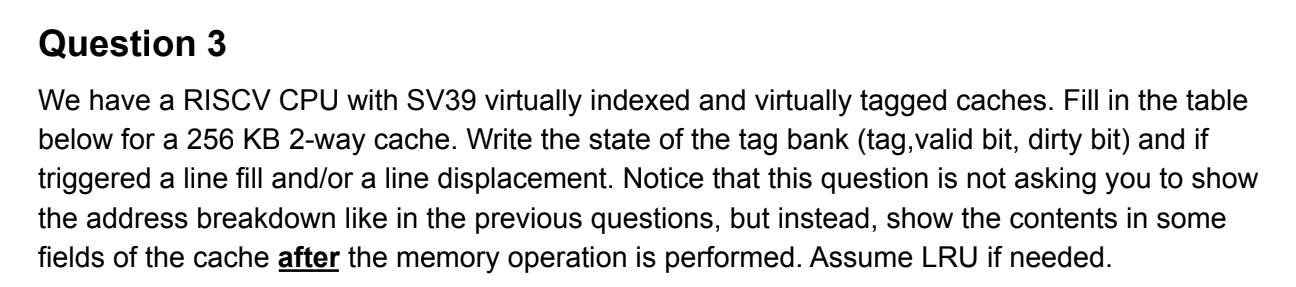
\includegraphics[scale=0.37]{q3_q.png}\\
\begin{proof}[Solution]
	\ \\
    \begin{tabular}{llrrrll}
	Memory Address & Tag   & \multicolumn{1}{l}{Valid bit} & \multicolumn{1}{l}{Dirty bit} & \multicolumn{1}{l}{Line Displacement} & Hit/Miss & Relevant index \\
	LD 0x1234AB22 & 0x91A & 1     & 0     & 1     & Miss  & 0xAB2 \\
	ST 0x1234AB20 & 0x91A & 1     & 1     & 0     & Hit   & 0xAB2 \\
	LD 0x1234D020 & 0x91A & 1     & 0     & 1     & Miss  & 0xD02 \\
	ST 0x1234D02F & 0x91A & 1     & 1     & 0     & Hit   & 0xD02 \\
	LD 0x1234AB26 & 0x91A & 1     & 1     & 0     & Hit   & 0xAB2 \\
	ST 0x1234AB33 & 0x91A & 1     & 1     & 1     & Miss  & 0xAB3 \\
	LD 0x1234D023 & 0x91A & 1     & 1     & 0     & Hit   & 0xD02 \\
	ST 0x1234D02B & 0x91A & 1     & 1     & 0     & Hit   & 0xD02 \\
	LD 0x1234AB22 & 0x91A & 1     & 1     & 0     & Hit   & 0xAB2 \\
	ST 0x1234AB28 & 0x91A & 1     & 1     & 0     & Hit   & 0xAB2 \\
	\end{tabular}\\
\end{proof}
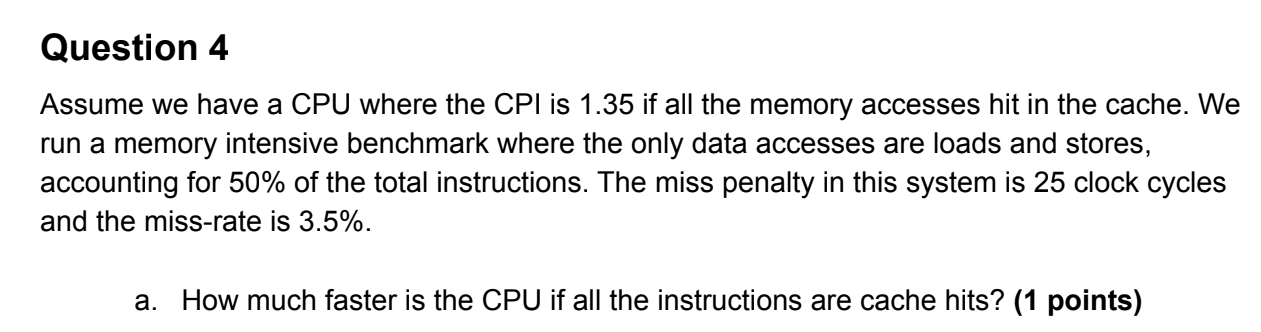
\includegraphics[scale=0.37]{q4_a.png}\\
\begin{proof}[Solution for a]
	$CPI_{old} = 1.35$\\
	$CPI_{new} = 1.35 + 0.5 * 0.035 * 25 = 1.7875$\\
	$speed\_up = CPI_{new} / CPI_{old} = 1.324$\\
\end{proof}
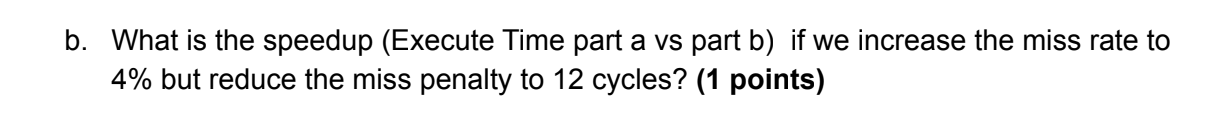
\includegraphics[scale=0.37]{q4_b.png}\\
\begin{proof}[Solution for b]
	$CPI_{old} = 1.7875$\\
	$CPI_{new} = 1.35 + 0.5 * 0.04 * 12 = 1.59$\\
	$speed\_up = CPI_{new} / CPI_{old} = 0.890$\\
\end{proof}
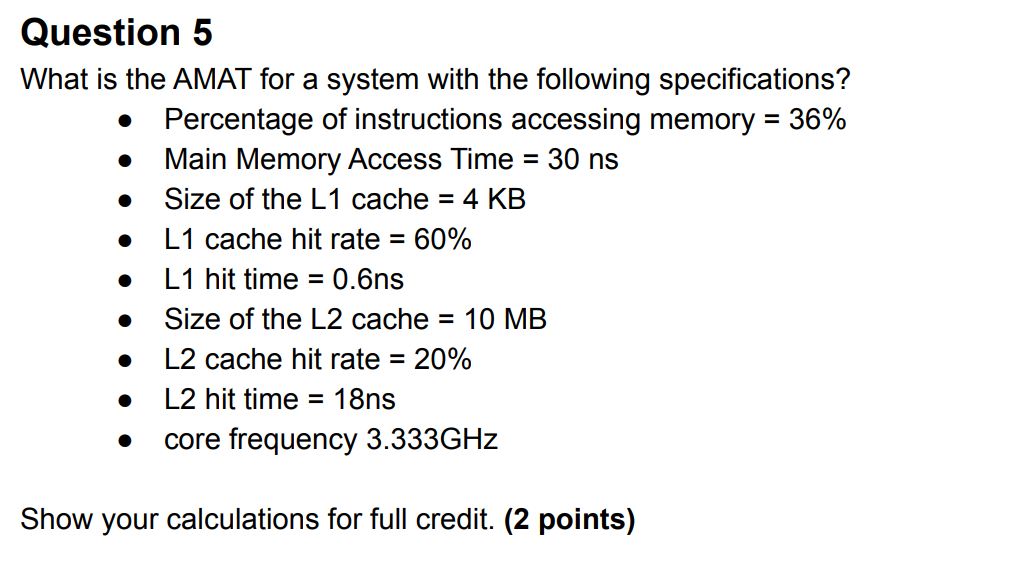
\includegraphics[scale=0.37]{q5_q.png}\\
\begin{proof}[Solution]
	$AMAT=0.6+0.4*18+0.4*0.8*30=17.4ns$
\end{proof}
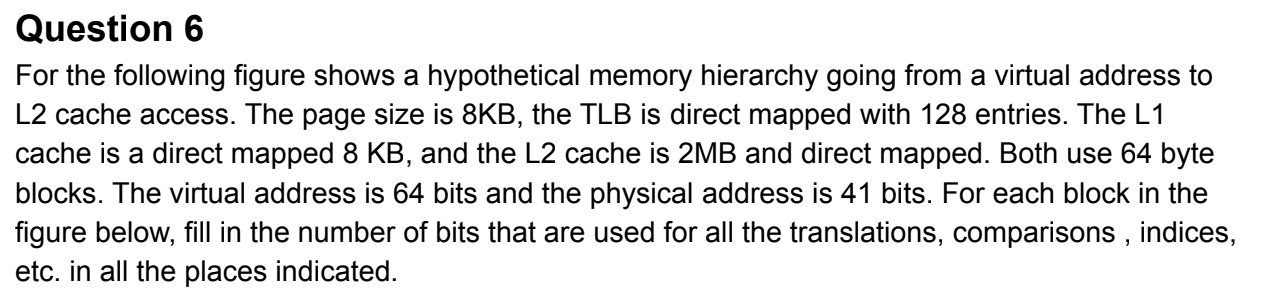
\includegraphics[scale=0.37]{q6_q.png}\\
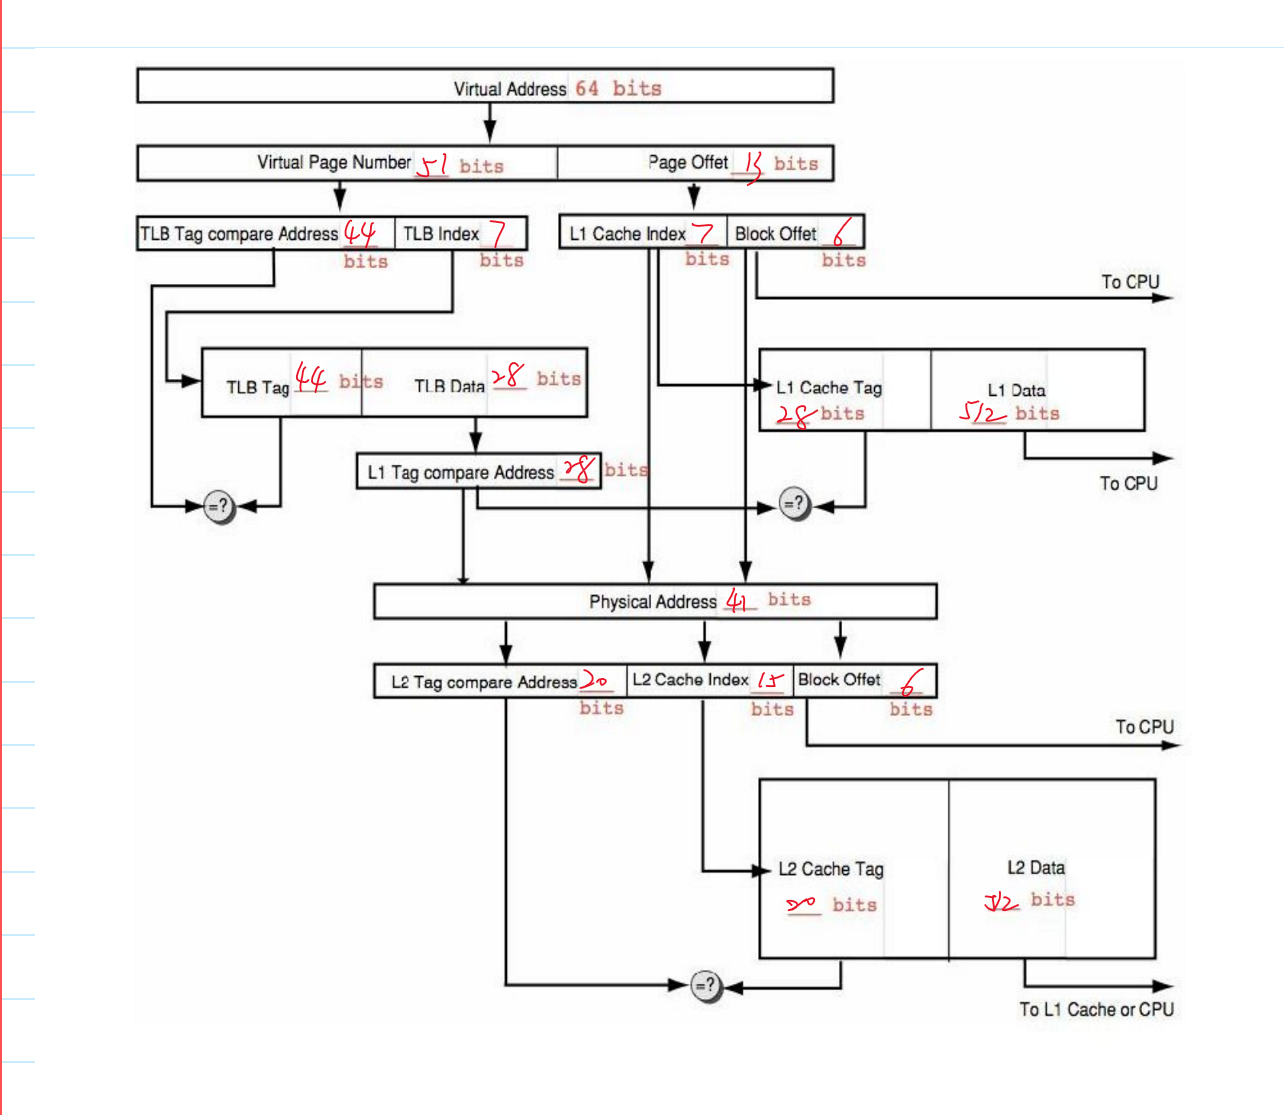
\includegraphics[scale=0.34]{q6.png}\\
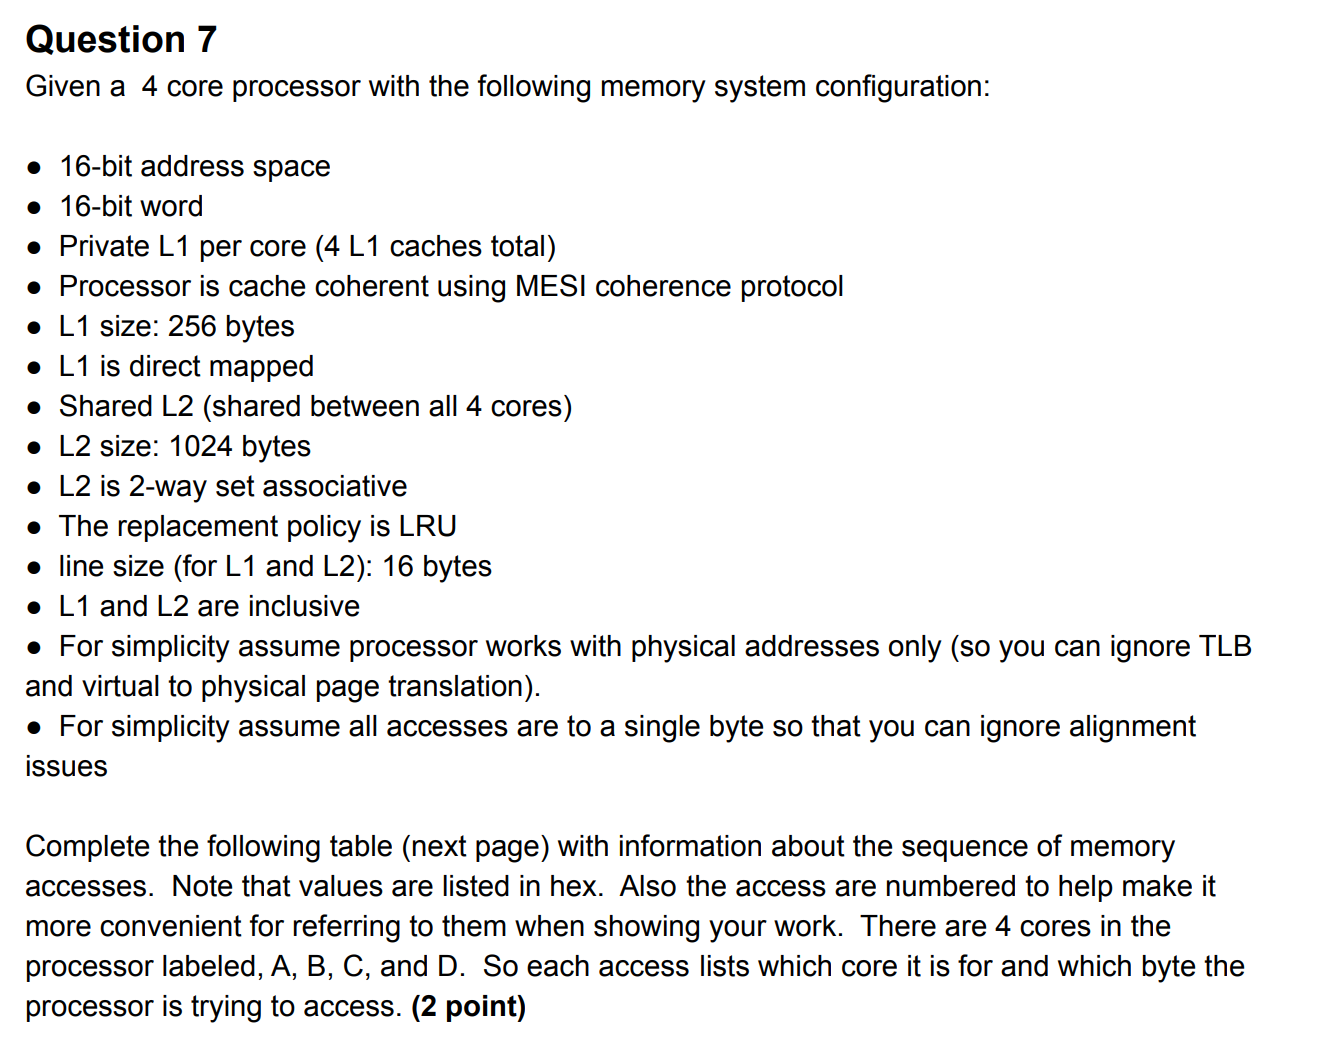
\includegraphics[scale=0.37]{q7_q.png}\\
\begin{proof}[Solution]
	\ \\
	    \begin{tabular}{rllllllll}
		\multicolumn{1}{l}{Access} & Core  & Type  & Address & L1    & L1 State & Bus   & L2    & L2 \\
		1     & A     & LD    & 0xFFA0 & Miss  & I-$>$E  & BR    & Miss  & I,I-$>$E,I \\
		2     & A     & ST    & 0xFFA0 & Hit   & E-$>$M  & --    & --    & -- \\
		3     & B     & ST    & 0xFFA2 & Miss  & I-$>$M  & BX,WB & Hit   & E,I-$>$M,I \\
		4     & A     & LD    & 0xFFA4 & Miss  & I-$>$S  & BR,WB & Hit   & M,I \\
		5     & C     & LD    & 0xFFAA & Miss  & I-$>$S  & BR    & Hit   & M,I \\
		6     & C     & ST    & 0x01AA & Miss  & S-$>$M  & BX    & Miss  & M,I-$>$M,E \\
		7     & D     & LD    & 0x01AA & Miss  & I-$>$S  & BR,WB & Hit   & M,E-$>$M,M \\
		8     & D     & LD    & 0x03AA & Miss  & S-$>$E  & BR    & Miss  & M,M-$>$E,M \\
		9     & A     & LD    & 0xFFA0 & Miss  & I-$>$E  & BR    & Miss  & E,M-$>$E,E \\
		10    & A     & ST    & 0x01AA & Miss  & I-$>$M  & BX    & Miss  & E,E \\
		11    & A     & LD    & 0xFFA2 & Miss  & M-$>$E  & BR    & Hit   & E,E-$>$M,E \\
		12    & C     & LD    & 0x01A4 & Miss  & I-$>$E  & BR    & Hit   & M,E \\
	\end{tabular}
\end{proof}
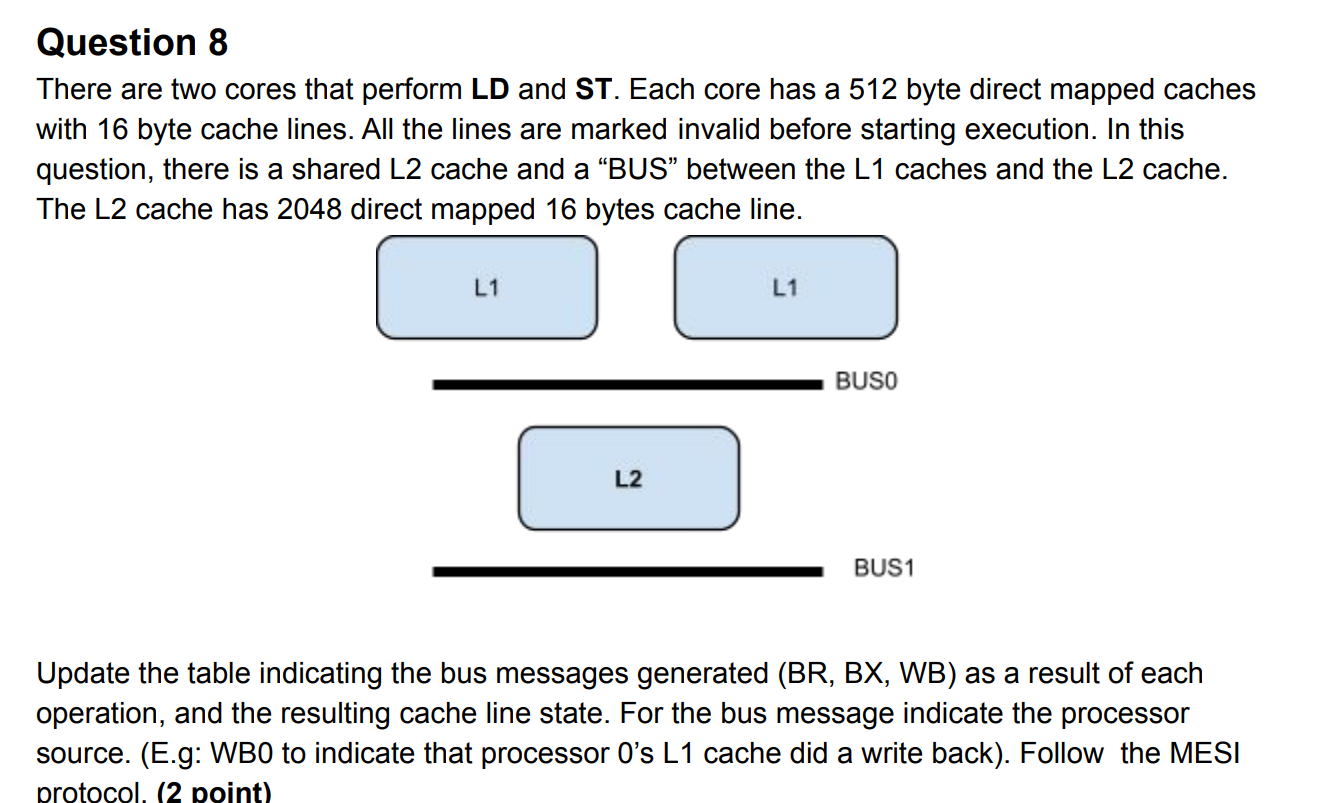
\includegraphics[scale=0.37]{q8.png}\\
\begin{proof}[Solution]
	\ \\
	    \begin{tabular}{llllll}
		Operation & Bus0  & Bus1  & P0 L1 & P1 L1 & L2 \\
		P0: ld [0x430] & BR0   & BR    & E     & I     & E \\
		P0: ld [0x438] & -     & -     & E     & I     & E \\
		P1: ld [0x300] & BR1   & BR    & I     & E     & E \\
		P0: st [0x300] & BX0   & -     & M     & I     & E \\
		P1: ld [0x300] & BR1, WB0 & -     & S     & S     & M \\
		P0: ld [0x430] & -     & -     & E     & I     & E \\
		P1: ld [0x400] & BR1   & BR    & I     & E     & E \\
		P0: st [0x400] & BX0   & -     & M     & I     & E \\
		P0: st [0x310] & BX1   & BX    & I     & M     & E \\
	\end{tabular}%
\end{proof}
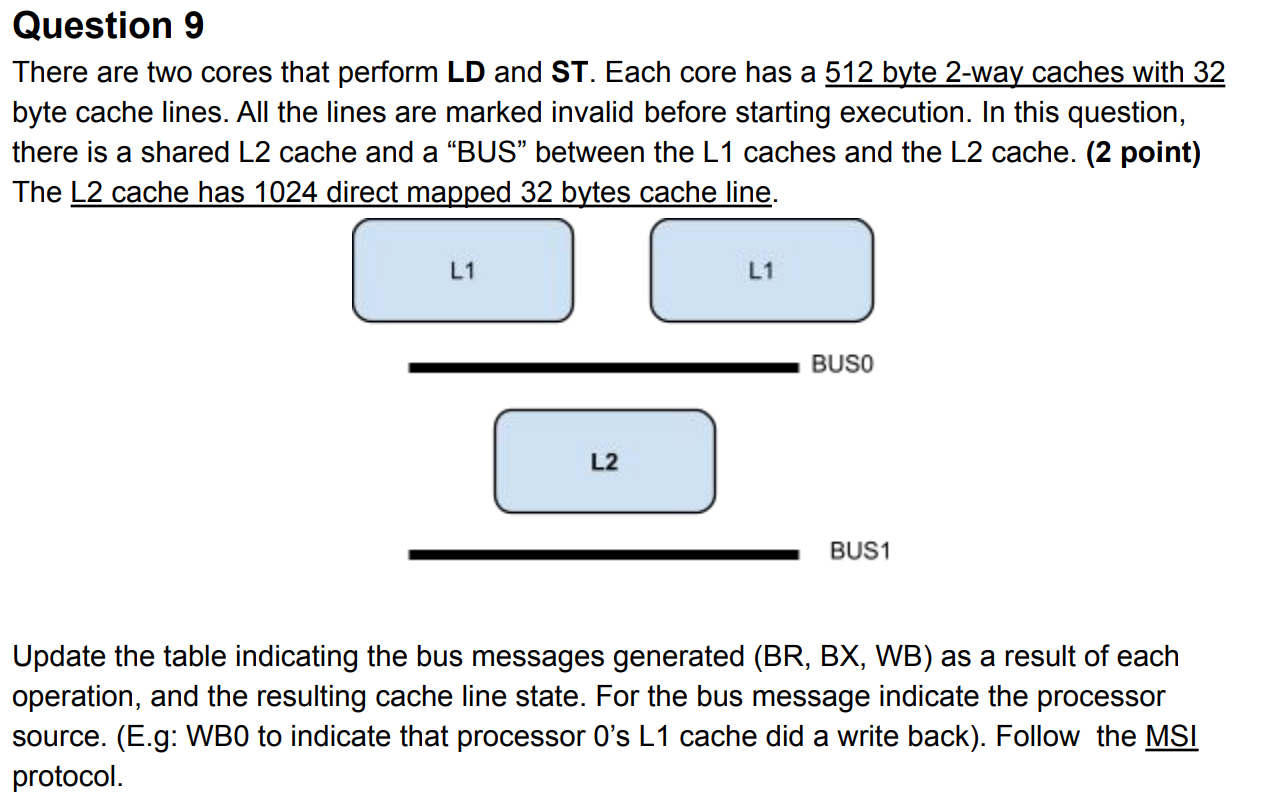
\includegraphics[scale=0.37]{q9.png}\\
\begin{proof}[Solution]
	\ \\
	\begin{tabular}{llllll}
		Operation & Bus0  & Bus1  & P0 L1 & P1 L1 & L2 \\
		P0: ld [0x430] & BR0   & BR    & S     & I     & S \\
		P0: ld [0x438] & -     & -     & S     & I     & S \\
		P1: ld [0x300] & BR1   & BR    & I     & S     & S \\
		P0: st [0x300] & BX0   & -     & M     & I     & S \\
		P1: ld [0x300] & BR1, WB0 & -     & S     & S     & M \\
		P0: ld [0x430] & -     & -     & S     & I     & S \\
		P1: ld [0x400] & BR1   & BR    & I     & S     & S \\
		P0: st [0x400] & BX0   & -     & M     & I     & S \\
		P0: st [0x310] & BX1   & -     & I     & M     & M \\
	\end{tabular}%
\end{proof}
\bigskip



\end{document}
